\documentclass{article}
\usepackage{url,color,xspace,verbatim,subfig,ctable,multirow,listings}
\usepackage[utf8]{inputenc}
\usepackage[T1]{fontenc}
\usepackage{txfonts}
\usepackage{rotating}
\usepackage{paralist}
\usepackage{subfig}
\usepackage{graphics}
\usepackage{enumitem}
\usepackage{times}
\usepackage{amssymb}
\usepackage[colorlinks=true]{hyperref}

% ==================================================

\graphicspath{{figs/}}
\urlstyle{sf}

% tikz stuff
\usepackage{tikz}
\usepackage{pgfplots}
\usetikzlibrary{shapes,positioning,calc,snakes,arrows,shapes}

\lstset{
  language=C,
  basicstyle=\ttfamily \small,
  flexiblecolumns=false,
  basewidth={0.5em,0.45em},
  boxpos=t,
}

\definecolor{skRed}{RGB}{155,25,25}
\newcommand{\stefan}[1]{
  {\color{skRed}[{\color{red}{SK}} #1]}}

% ==================================================

\begin{document}

\title{Replication on multicore considering hierarchy and
  characteristics of the network}

% email address
\newcommand{\eaddr}{stefan.kaestle@inf.ethz.ch}
\newcommand{\email}{\href{mailto:\eaddr}{\eaddr}}

\author{Stefan Kaestle\\
  \email \\
  Systems Group, ETH Zurich}

\maketitle

\paragraph{What do you want to enable?} Increase algorithm performance
on multicores by applying distributed principles, particularly
replication. The challenge then is to guarantee consistency. Previous
work was using primary copy protocols to do that~\cite{Wiesmann2000}, a
passive replication scheme (i.e.\ nodes do not have to contact all
replicas). They do that because they claim that it is not suitable for
clients to know about replication details. An atomic broadcast is
often used as foundation of such algorithms. It guarantees in reliable
delivery of messages to every node.

\paragraph{What problem are you solving, and why is it hard?} Three problems:
\begin{description}
\item[placement] machine dependent
\item[consistency] need to consider machine \emph{characteristics};
  multicores are \emph{different} from classical distributed systems.
\item[machine characteristics] diverse, fast changing, complex. One
  example is the batch size for sending a broadcast.
\end{description}

\paragraph{What's the related work?} People do replication to deal
with scalability challenges on multicores, e.g.\
databases~\cite{Salomie2011, Wiesmann2000} and operating
systems~\cite{fos:osr09, tornado:osdi99, barrelfish:sosp09}. But they
don't to it properly. They do not consider machine characteristics or
apply the wrong distributed technologies.

\paragraph{What new idea(s) will solve the problems?} We do a
hierarchical group communication, which implements an atomic
broadcast on multicore machines. It has message complexity of
$O(\frac{n}{2})$ and time complexity $O(log(n))$ as opposed to
algorithms from traditional distributed systems having $O(2)$ message
complexity and $O(n)$ time complexity. %
\\
{\footnotesize Example: sequential consistency on shared memory, do
  not really need to have primary backup.}

\paragraph{How will you go about it?} Replicas on NUMA domains, show
that overall throughput is higher. Then, use a quorum based approach for
consistency. Consistency by doing a hierarchical group communication
approach instead of sequential send from same nodes.

\paragraph{How will you know and show it works?} Database?
Microbenchmark? Compare to primary backup, which is typically
used. Measure time required to apply an update.

\paragraph{What is your hypothesis?} We can do much better if machine
characteristics are considered.

%%%%%%%%%%%%%%%%%%%%%%%%%%%%%%%%%%%%%%%%%%%%%%%%%%
\subsection{Mechanisms}

\subsubsection{Aggregation}

Similarly to what has been done in wireless sensor networks (where it
also matters to reduce the number of messages, but other reasons:
power consumption), we can do aggregation in nodes. In difference to
traditional distributed systems, this works, because it is easy to
deploy custom software on every node in the network. Classical
distributed systems do not typically allow this. Furthermore, reducing
the number of messages at the price of higher complexity does not make
sense there.

Examples for aggregation: number of nodes agreeing to something, find
capabilities (concatenate core ids). 

Open questions: How does this work with several senders (everyone is
potentially a sender). Maybe something like in navigation
systems. Every node has an entry point, which forwards the
messages. Nodes are then clustered \ldots

%%%%%%%%%%%%%%%%%%%%%%%%%%%%%%%%%%%%%%%%%%%%%%%%%%
\subsection{Implementation}

Build a tree. Every node has parents and children (except for the root
and the leafs). The number of children does not really matter for the
algorithm. In the init phase, we construct the tree (e.g. broadcast:
one root node, all other nodes are children of the root node,
multicast: every node has two children, NUMA tree: two layers, two
different implementations?

Reducing the number of children also helps in select. It reduces the
number of ``channels'' to poll, and therefore the latency of detecting
messages. Instead of 

%%%%%%%%%%%%%%%%%%%%%%%%%%%%%%%%%%%%%%%%%%%%%%%%%%
\subsection{Experimental results}

\paragraph{Current numbers}

\begin{table}[htb]
  \centering
  \begin{tabular}{lrrrr}
    \toprule
    broadcast algorithm & \multicolumn{2}{c}{nos5} & \multicolumn{2}{c}{gruyere} \\
      & cycles & error & cycles & error \\
    \midrule
    sequential &  4096.1 &  105.2 & 136751.9 &   3061.5 \\
    batch      &  2408.0 &  181.9 &  57360.8 &   5271.5 \\
    \bottomrule
  \end{tabular}
  \caption{Broadcast measurements}
  \label{tab:bc_measurements}
\end{table}

\paragraph{Tree setup} \stefan{describe}

\paragraph{Measurements to do next} %
\begin{itemize}
\item Increase number of cores to talk to in every round. Use a
  separate waitsets, so that we don't have additional overhead from
  the bindings not used in each concrete measurement.
\item Play with batching. Incrementally increase the number of
  messages send in a batch. I assume this is machine specific, which
  means, that this is something programmers do not want to deal
  with. We measure this at dynamically at run-time and find the right
  batch size.
\end{itemize}

\paragraph{Minimal cost of sending a tree-broadcast} %
Plot~\ref{pgfplot:201303141819} shows the minimal cost of flooding a
sub-tree. The group communication is based on a binary tree. Core 0 is
the root, cores 1 and 2 are its children etc.

The average cost is really high (so something is wrong with my
code). But the minimal numbers show what is possible. The numbers
achieved are easily explainable. The cost is increasing
logarithmic with the number of nodes reached by the broadcast (as
expected). Every level in the tree adds an additional 3500 cycles to
the tree. Node 0 takes significantly longer. I don't know yet why that
is.

\begin{figure}
  \caption{Plot}
  \label{pgfplot:201303141819}
  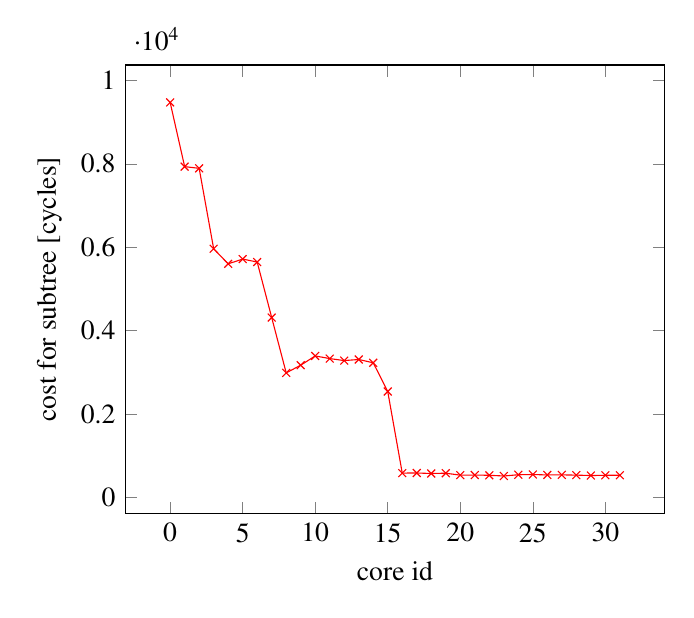
\begin{tikzpicture}
    \begin{axis}[
      xlabel=core id,
      ylabel={cost for subtree [cycles]}]
    \addplot[color=red,mark=x] coordinates {
      (0,9475.0)
      (1,7935.0)
      (2,7894.0)
      (3,5965.0)
      (4,5604.0)
      (5,5718.0)
      (6,5647.0)
      (7,4316.0)
      (8,2989.0)
      (9,3173.0)
      (10,3395.0)
      (11,3332.0)
      (12,3284.0)
      (13,3310.0)
      (14,3231.0)
      (15,2542.0)
      (16,586.0)
      (17,588.0)
      (18,576.0)
      (19,583.0)
      (20,536.0)
      (21,539.0)
      (22,533.0)
      (23,516.0)
      (24,546.0)
      (25,552.0)
      (26,541.0)
      (27,543.0)
      (28,537.0)
      (29,527.0)
      (30,533.0)
      (31,534.0)
    };
    \end{axis}
  \end{tikzpicture}

\end{figure}
  
\begin{figure}
  % Start of code
% \begin{tikzpicture}[anchor=mid,>=latex',line join=bevel,]
\begin{tikzpicture}[>=latex',line join=bevel,scale=.35]
  \pgfsetlinewidth{1bp}
%%
\pgfsetcolor{black}
  % Edge: 15 -> 31
  \draw [->] (27bp,74.327bp) .. controls (27bp,66.264bp) and (27bp,56.648bp)  .. (27bp,37.667bp);
  % Edge: 9 -> 19
  \draw [->] (459bp,148.33bp) .. controls (459bp,140.26bp) and (459bp,130.65bp)  .. (459bp,111.67bp);
  % Edge: 14 -> 30
  \draw [->] (1050.3bp,151.31bp) .. controls (1060.4bp,140.94bp) and (1073.7bp,127.18bp)  .. (1092bp,108.42bp);
  % Edge: 14 -> 29
  \draw [->] (1035bp,148.33bp) .. controls (1035bp,140.26bp) and (1035bp,130.65bp)  .. (1035bp,111.67bp);
  % Edge: 11 -> 23
  \draw [->] (659.73bp,151.31bp) .. controls (649.64bp,140.94bp) and (636.25bp,127.18bp)  .. (618bp,108.42bp);
  % Edge: 7 -> 15
  \draw [->] (83.731bp,151.31bp) .. controls (73.64bp,140.94bp) and (60.253bp,127.18bp)  .. (42bp,108.42bp);
  % Edge: 0 -> 2
  \draw [->] (588.87bp,377.76bp) .. controls (613.22bp,365.25bp) and (652.76bp,344.93bp)  .. (689.4bp,326.1bp);
  % Edge: 10 -> 22
  \draw [->] (387bp,148.33bp) .. controls (387bp,140.26bp) and (387bp,130.65bp)  .. (387bp,111.67bp);
  % Edge: 13 -> 28
  \draw [->] (935.71bp,149.09bp) .. controls (939.96bp,140.36bp) and (945.15bp,129.68bp)  .. (954.37bp,110.75bp);
  % Edge: 1 -> 3
  \draw [->] (398.64bp,306.66bp) .. controls (360.05bp,293.43bp) and (284.76bp,267.64bp)  .. (231.27bp,249.31bp);
  % Edge: 6 -> 14
  \draw [->] (946.31bp,227.77bp) .. controls (963.36bp,216.09bp) and (988.4bp,198.93bp)  .. (1015.9bp,180.12bp);
  % Edge: 3 -> 8
  \draw [->] (207bp,222.33bp) .. controls (207bp,214.26bp) and (207bp,204.65bp)  .. (207bp,185.67bp);
  % Edge: 13 -> 27
  \draw [->] (918.29bp,149.09bp) .. controls (914.04bp,140.36bp) and (908.85bp,129.68bp)  .. (899.63bp,110.75bp);
  % Edge: 10 -> 21
  \draw [->] (371.73bp,151.31bp) .. controls (361.64bp,140.94bp) and (348.25bp,127.18bp)  .. (330bp,108.42bp);
  % Edge: 12 -> 26
  \draw [->] (762.27bp,151.31bp) .. controls (772.36bp,140.94bp) and (785.75bp,127.18bp)  .. (804bp,108.42bp);
  % Edge: 3 -> 7
  \draw [->] (187.69bp,227.77bp) .. controls (170.64bp,216.09bp) and (145.6bp,198.93bp)  .. (118.14bp,180.12bp);
  % Edge: 5 -> 12
  \draw [->] (719.71bp,223.09bp) .. controls (723.96bp,214.36bp) and (729.15bp,203.68bp)  .. (738.37bp,184.75bp);
  % Edge: 9 -> 20
  \draw [->] (474.27bp,151.31bp) .. controls (484.36bp,140.94bp) and (497.75bp,127.18bp)  .. (516bp,108.42bp);
  % Edge: 1 -> 4
  \draw [->] (423bp,296.33bp) .. controls (423bp,288.26bp) and (423bp,278.65bp)  .. (423bp,259.67bp);
  % Edge: 0 -> 1
  \draw [->] (545.13bp,377.76bp) .. controls (520.78bp,365.25bp) and (481.24bp,344.93bp)  .. (444.6bp,326.1bp);
  % Edge: 2 -> 5
  \draw [->] (711bp,296.33bp) .. controls (711bp,288.26bp) and (711bp,278.65bp)  .. (711bp,259.67bp);
  % Edge: 11 -> 24
  \draw [->] (675bp,148.33bp) .. controls (675bp,140.26bp) and (675bp,130.65bp)  .. (675bp,111.67bp);
  % Edge: 4 -> 10
  \draw [->] (414.29bp,223.09bp) .. controls (410.04bp,214.36bp) and (404.85bp,203.68bp)  .. (395.63bp,184.75bp);
  % Edge: 12 -> 25
  \draw [->] (747bp,148.33bp) .. controls (747bp,140.26bp) and (747bp,130.65bp)  .. (747bp,111.67bp);
  % Edge: 8 -> 17
  \draw [->] (198.29bp,149.09bp) .. controls (194.04bp,140.36bp) and (188.85bp,129.68bp)  .. (179.63bp,110.75bp);
  % Edge: 6 -> 13
  \draw [->] (927bp,222.33bp) .. controls (927bp,214.26bp) and (927bp,204.65bp)  .. (927bp,185.67bp);
  % Edge: 5 -> 11
  \draw [->] (702.29bp,223.09bp) .. controls (698.04bp,214.36bp) and (692.85bp,203.68bp)  .. (683.63bp,184.75bp);
  % Edge: 7 -> 16
  \draw [->] (99bp,148.33bp) .. controls (99bp,140.26bp) and (99bp,130.65bp)  .. (99bp,111.67bp);
  % Edge: 2 -> 6
  \draw [->] (735.36bp,306.66bp) .. controls (773.95bp,293.43bp) and (849.24bp,267.64bp)  .. (902.73bp,249.31bp);
  % Edge: 8 -> 18
  \draw [->] (215.71bp,149.09bp) .. controls (219.96bp,140.36bp) and (225.15bp,129.68bp)  .. (234.37bp,110.75bp);
  % Edge: 4 -> 9
  \draw [->] (431.71bp,223.09bp) .. controls (435.96bp,214.36bp) and (441.15bp,203.68bp)  .. (450.37bp,184.75bp);
  % Node: 24
\begin{scope}
  \definecolor{strokecol}{rgb}{0.0,0.0,0.0};
  \pgfsetstrokecolor{strokecol}
  \draw (675bp,93bp) ellipse (27bp and 18bp);
  \draw (675bp,93bp) node {24};
\end{scope}
  % Node: 25
\begin{scope}
  \definecolor{strokecol}{rgb}{0.0,0.0,0.0};
  \pgfsetstrokecolor{strokecol}
  \draw (747bp,93bp) ellipse (27bp and 18bp);
  \draw (747bp,93bp) node {25};
\end{scope}
  % Node: 26
\begin{scope}
  \definecolor{strokecol}{rgb}{0.0,0.0,0.0};
  \pgfsetstrokecolor{strokecol}
  \draw (819bp,93bp) ellipse (27bp and 18bp);
  \draw (819bp,93bp) node {26};
\end{scope}
  % Node: 27
\begin{scope}
  \definecolor{strokecol}{rgb}{0.0,0.0,0.0};
  \pgfsetstrokecolor{strokecol}
  \draw (891bp,93bp) ellipse (27bp and 18bp);
  \draw (891bp,93bp) node {27};
\end{scope}
  % Node: 20
\begin{scope}
  \definecolor{strokecol}{rgb}{0.0,0.0,0.0};
  \pgfsetstrokecolor{strokecol}
  \draw (531bp,93bp) ellipse (27bp and 18bp);
  \draw (531bp,93bp) node {20};
\end{scope}
  % Node: 21
\begin{scope}
  \definecolor{strokecol}{rgb}{0.0,0.0,0.0};
  \pgfsetstrokecolor{strokecol}
  \draw (315bp,93bp) ellipse (27bp and 18bp);
  \draw (315bp,93bp) node {21};
\end{scope}
  % Node: 22
\begin{scope}
  \definecolor{strokecol}{rgb}{0.0,0.0,0.0};
  \pgfsetstrokecolor{strokecol}
  \draw (387bp,93bp) ellipse (27bp and 18bp);
  \draw (387bp,93bp) node {22};
\end{scope}
  % Node: 23
\begin{scope}
  \definecolor{strokecol}{rgb}{0.0,0.0,0.0};
  \pgfsetstrokecolor{strokecol}
  \draw (603bp,93bp) ellipse (27bp and 18bp);
  \draw (603bp,93bp) node {23};
\end{scope}
  % Node: 28
\begin{scope}
  \definecolor{strokecol}{rgb}{0.0,0.0,0.0};
  \pgfsetstrokecolor{strokecol}
  \draw (963bp,93bp) ellipse (27bp and 18bp);
  \draw (963bp,93bp) node {28};
\end{scope}
  % Node: 29
\begin{scope}
  \definecolor{strokecol}{rgb}{0.0,0.0,0.0};
  \pgfsetstrokecolor{strokecol}
  \draw (1035bp,93bp) ellipse (27bp and 18bp);
  \draw (1035bp,93bp) node {29};
\end{scope}
  % Node: 1
\begin{scope}
  \definecolor{strokecol}{rgb}{0.0,0.0,0.0};
  \pgfsetstrokecolor{strokecol}
  \draw (423bp,315bp) ellipse (27bp and 18bp);
  \draw (423bp,315bp) node {1};
\end{scope}
  % Node: 0
\begin{scope}
  \definecolor{strokecol}{rgb}{0.0,0.0,0.0};
  \pgfsetstrokecolor{strokecol}
  \draw (567bp,389bp) ellipse (27bp and 18bp);
  \draw (567bp,389bp) node {0};
\end{scope}
  % Node: 3
\begin{scope}
  \definecolor{strokecol}{rgb}{0.0,0.0,0.0};
  \pgfsetstrokecolor{strokecol}
  \draw (207bp,241bp) ellipse (27bp and 18bp);
  \draw (207bp,241bp) node {3};
\end{scope}
  % Node: 2
\begin{scope}
  \definecolor{strokecol}{rgb}{0.0,0.0,0.0};
  \pgfsetstrokecolor{strokecol}
  \draw (711bp,315bp) ellipse (27bp and 18bp);
  \draw (711bp,315bp) node {2};
\end{scope}
  % Node: 5
\begin{scope}
  \definecolor{strokecol}{rgb}{0.0,0.0,0.0};
  \pgfsetstrokecolor{strokecol}
  \draw (711bp,241bp) ellipse (27bp and 18bp);
  \draw (711bp,241bp) node {5};
\end{scope}
  % Node: 4
\begin{scope}
  \definecolor{strokecol}{rgb}{0.0,0.0,0.0};
  \pgfsetstrokecolor{strokecol}
  \draw (423bp,241bp) ellipse (27bp and 18bp);
  \draw (423bp,241bp) node {4};
\end{scope}
  % Node: 7
\begin{scope}
  \definecolor{strokecol}{rgb}{0.0,0.0,0.0};
  \pgfsetstrokecolor{strokecol}
  \draw (99bp,167bp) ellipse (27bp and 18bp);
  \draw (99bp,167bp) node {7};
\end{scope}
  % Node: 6
\begin{scope}
  \definecolor{strokecol}{rgb}{0.0,0.0,0.0};
  \pgfsetstrokecolor{strokecol}
  \draw (927bp,241bp) ellipse (27bp and 18bp);
  \draw (927bp,241bp) node {6};
\end{scope}
  % Node: 9
\begin{scope}
  \definecolor{strokecol}{rgb}{0.0,0.0,0.0};
  \pgfsetstrokecolor{strokecol}
  \draw (459bp,167bp) ellipse (27bp and 18bp);
  \draw (459bp,167bp) node {9};
\end{scope}
  % Node: 8
\begin{scope}
  \definecolor{strokecol}{rgb}{0.0,0.0,0.0};
  \pgfsetstrokecolor{strokecol}
  \draw (207bp,167bp) ellipse (27bp and 18bp);
  \draw (207bp,167bp) node {8};
\end{scope}
  % Node: 11
\begin{scope}
  \definecolor{strokecol}{rgb}{0.0,0.0,0.0};
  \pgfsetstrokecolor{strokecol}
  \draw (675bp,167bp) ellipse (27bp and 18bp);
  \draw (675bp,167bp) node {11};
\end{scope}
  % Node: 10
\begin{scope}
  \definecolor{strokecol}{rgb}{0.0,0.0,0.0};
  \pgfsetstrokecolor{strokecol}
  \draw (387bp,167bp) ellipse (27bp and 18bp);
  \draw (387bp,167bp) node {10};
\end{scope}
  % Node: 13
\begin{scope}
  \definecolor{strokecol}{rgb}{0.0,0.0,0.0};
  \pgfsetstrokecolor{strokecol}
  \draw (927bp,167bp) ellipse (27bp and 18bp);
  \draw (927bp,167bp) node {13};
\end{scope}
  % Node: 12
\begin{scope}
  \definecolor{strokecol}{rgb}{0.0,0.0,0.0};
  \pgfsetstrokecolor{strokecol}
  \draw (747bp,167bp) ellipse (27bp and 18bp);
  \draw (747bp,167bp) node {12};
\end{scope}
  % Node: 15
\begin{scope}
  \definecolor{strokecol}{rgb}{0.0,0.0,0.0};
  \pgfsetstrokecolor{strokecol}
  \draw (27bp,93bp) ellipse (27bp and 18bp);
  \draw (27bp,93bp) node {15};
\end{scope}
  % Node: 14
\begin{scope}
  \definecolor{strokecol}{rgb}{0.0,0.0,0.0};
  \pgfsetstrokecolor{strokecol}
  \draw (1035bp,167bp) ellipse (27bp and 18bp);
  \draw (1035bp,167bp) node {14};
\end{scope}
  % Node: 17
\begin{scope}
  \definecolor{strokecol}{rgb}{0.0,0.0,0.0};
  \pgfsetstrokecolor{strokecol}
  \draw (171bp,93bp) ellipse (27bp and 18bp);
  \draw (171bp,93bp) node {17};
\end{scope}
  % Node: 16
\begin{scope}
  \definecolor{strokecol}{rgb}{0.0,0.0,0.0};
  \pgfsetstrokecolor{strokecol}
  \draw (99bp,93bp) ellipse (27bp and 18bp);
  \draw (99bp,93bp) node {16};
\end{scope}
  % Node: 19
\begin{scope}
  \definecolor{strokecol}{rgb}{0.0,0.0,0.0};
  \pgfsetstrokecolor{strokecol}
  \draw (459bp,93bp) ellipse (27bp and 18bp);
  \draw (459bp,93bp) node {19};
\end{scope}
  % Node: 18
\begin{scope}
  \definecolor{strokecol}{rgb}{0.0,0.0,0.0};
  \pgfsetstrokecolor{strokecol}
  \draw (243bp,93bp) ellipse (27bp and 18bp);
  \draw (243bp,93bp) node {18};
\end{scope}
  % Node: 31
\begin{scope}
  \definecolor{strokecol}{rgb}{0.0,0.0,0.0};
  \pgfsetstrokecolor{strokecol}
  \draw (27bp,19bp) ellipse (27bp and 18bp);
  \draw (27bp,19bp) node {31};
\end{scope}
  % Node: 30
\begin{scope}
  \definecolor{strokecol}{rgb}{0.0,0.0,0.0};
  \pgfsetstrokecolor{strokecol}
  \draw (1107bp,93bp) ellipse (27bp and 18bp);
  \draw (1107bp,93bp) node {30};
\end{scope}
%
\end{tikzpicture}
% End of code




  \caption{Tree of cores for broadcast on gruyere}
\end{figure}

Plot~\ref{pgfplot:201303071512} shows some weirdness on gruyere. The
cost of the broadcast seems to be growing over time. No clue why. 

\begin{figure}
  \caption{Sequential broadcast on gruyere. In every round, we send a
    request to every other core in the system and wait for an ACK
    before sending the next message. For the table we only use the
    results between round 450 and 600, as these seem to be most stable.}
  \label{pgfplot:201303071512}
  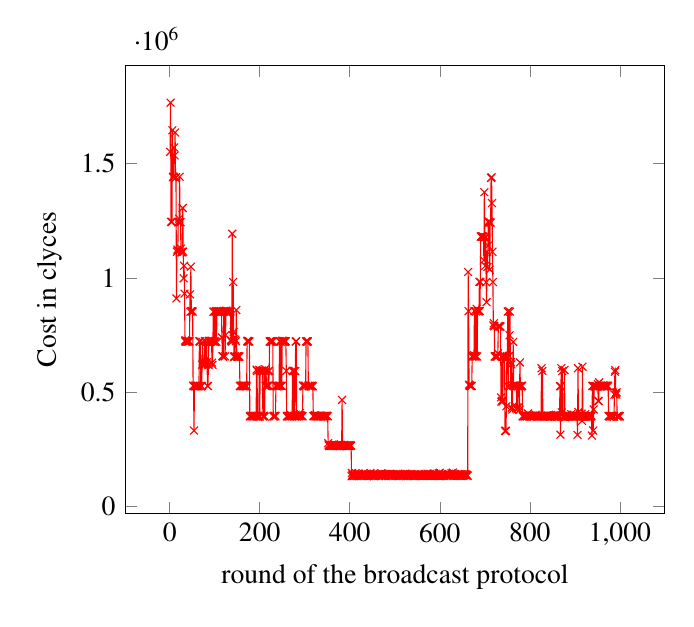
\begin{tikzpicture}
    \begin{axis}[
      xlabel=round of the broadcast protocol,
      ylabel=Cost in clyces]
    \addplot[color=red,mark=x] coordinates {
      (1,1551986)
      (2,1767396)
      (3,1245103)
      (4,1245218)
      (5,1245153)
      (6,1646349)
      (7,1440759)
      (8,1443429)
      (9,1442761)
      (10,1571085)
      (11,1536129)
      (12,1636917)
      (13,1438167)
      (14,1440759)
      (15,910123)
      (16,1114930)
      (17,1124375)
      (18,1119390)
      (19,1243732)
      (20,1244306)
      (21,1259213)
      (22,1443211)
      (23,1243931)
      (24,1243979)
      (25,1128069)
      (26,1112171)
      (27,1114456)
      (28,1111746)
      (29,1306131)
      (30,1115393)
      (31,998171)
      (32,1053532)
      (33,931168)
      (34,722147)
      (35,727529)
      (36,722582)
      (37,720077)
      (38,722550)
      (39,722833)
      (40,722295)
      (41,722271)
      (42,721841)
      (43,722681)
      (44,722120)
      (45,927799)
      (46,852087)
      (47,1049032)
      (48,854705)
      (49,854594)
      (50,854415)
      (51,851773)
      (52,528100)
      (53,526252)
      (54,331609)
      (55,525972)
      (56,527791)
      (57,525013)
      (58,527771)
      (59,526273)
      (60,526060)
      (61,527942)
      (62,524838)
      (63,528330)
      (64,526166)
      (65,526141)
      (66,722370)
      (67,720255)
      (68,723332)
      (69,525783)
      (70,526481)
      (71,526253)
      (72,620169)
      (73,720392)
      (74,629440)
      (75,621080)
      (76,626836)
      (77,619148)
      (78,723892)
      (79,627084)
      (80,621107)
      (81,720051)
      (82,719931)
      (83,631664)
      (84,527006)
      (85,526051)
      (86,619123)
      (87,724616)
      (88,718910)
      (89,723856)
      (90,719999)
      (91,719672)
      (92,722974)
      (93,724861)
      (94,628968)
      (95,619522)
      (96,721813)
      (97,852169)
      (98,721893)
      (99,852406)
      (100,720204)
      (101,722494)
      (102,852331)
      (103,854355)
      (104,719880)
      (105,853793)
      (106,852080)
      (107,851943)
      (108,851788)
      (109,852059)
      (110,854511)
      (111,850536)
      (112,852182)
      (113,851802)
      (114,853831)
      (115,851472)
      (116,739344)
      (117,658076)
      (118,655828)
      (119,655822)
      (120,854260)
      (121,853894)
      (122,854486)
      (123,656502)
      (124,749498)
      (125,852076)
      (126,856861)
      (127,850544)
      (128,852049)
      (129,852341)
      (130,852712)
      (131,852146)
      (132,850903)
      (133,851967)
      (134,852780)
      (135,852076)
      (136,727925)
      (137,724363)
      (138,720062)
      (139,1193351)
      (140,748602)
      (141,981909)
      (142,763277)
      (143,654200)
      (144,656066)
      (145,656048)
      (146,729961)
      (147,722542)
      (148,859399)
      (149,655934)
      (150,655949)
      (151,658030)
      (152,654398)
      (153,657198)
      (154,655456)
      (155,655268)
      (156,526249)
      (157,527688)
      (158,527207)
      (159,526946)
      (160,526017)
      (161,528073)
      (162,528396)
      (163,525670)
      (164,526599)
      (165,528782)
      (166,525414)
      (167,528107)
      (168,525912)
      (169,525756)
      (170,528411)
      (171,525322)
      (172,722616)
      (173,724860)
      (174,721079)
      (175,722461)
      (176,722266)
      (177,721816)
      (178,393371)
      (179,395649)
      (180,395638)
      (181,395527)
      (182,393666)
      (183,395420)
      (184,395040)
      (185,394267)
      (186,395767)
      (187,394352)
      (188,393797)
      (189,395632)
      (190,395262)
      (191,393974)
      (192,396372)
      (193,598502)
      (194,592417)
      (195,393293)
      (196,394391)
      (197,396622)
      (198,393176)
      (199,597056)
      (200,393355)
      (201,593393)
      (202,592047)
      (203,592849)
      (204,592598)
      (205,592270)
      (206,593673)
      (207,394002)
      (208,393833)
      (209,396331)
      (210,592911)
      (211,392931)
      (212,599835)
      (213,525657)
      (214,591905)
      (215,525862)
      (216,527737)
      (217,525340)
      (218,528327)
      (219,591016)
      (220,528080)
      (221,592661)
      (222,721191)
      (223,722724)
      (224,722422)
      (225,722672)
      (226,719989)
      (227,722225)
      (228,722864)
      (229,722473)
      (230,393581)
      (231,395910)
      (232,393642)
      (233,395732)
      (234,395902)
      (235,394154)
      (236,526307)
      (237,528490)
      (238,525042)
      (239,528588)
      (240,525990)
      (241,526272)
      (242,526626)
      (243,527940)
      (244,721755)
      (245,528001)
      (246,722597)
      (247,720233)
      (248,527118)
      (249,527294)
      (250,724618)
      (251,724713)
      (252,720765)
      (253,722056)
      (254,722577)
      (255,722772)
      (256,720507)
      (257,722467)
      (258,723005)
      (259,592526)
      (260,393793)
      (261,394469)
      (262,396752)
      (263,394118)
      (264,393868)
      (265,395856)
      (266,393674)
      (267,396511)
      (268,394449)
      (269,395792)
      (270,399596)
      (271,394775)
      (272,393389)
      (273,593484)
      (274,592001)
      (275,395507)
      (276,592660)
      (277,396265)
      (278,394457)
      (279,592227)
      (280,721393)
      (281,723050)
      (282,393306)
      (283,395775)
      (284,394159)
      (285,396313)
      (286,399344)
      (287,394479)
      (288,394379)
      (289,408014)
      (290,398570)
      (291,395692)
      (292,396189)
      (293,394063)
      (294,395958)
      (295,393370)
      (296,528702)
      (297,525860)
      (298,525385)
      (299,527760)
      (300,526940)
      (301,526111)
      (302,527513)
      (303,722243)
      (304,722117)
      (305,720228)
      (306,722548)
      (307,722071)
      (308,528088)
      (309,526027)
      (310,525893)
      (311,526562)
      (312,526937)
      (313,527893)
      (314,525923)
      (315,525467)
      (316,528429)
      (317,526019)
      (318,525586)
      (319,394847)
      (320,393945)
      (321,396827)
      (322,395724)
      (323,398628)
      (324,394323)
      (325,396169)
      (326,394231)
      (327,393699)
      (328,396441)
      (329,393352)
      (330,395732)
      (331,395786)
      (332,393573)
      (333,396392)
      (334,394880)
      (335,394102)
      (336,396260)
      (337,393398)
      (338,395615)
      (339,395669)
      (340,393982)
      (341,393782)
      (342,395937)
      (343,394268)
      (344,394776)
      (345,395062)
      (346,395549)
      (347,395469)
      (348,395599)
      (349,396300)
      (350,395481)
      (351,394105)
      (352,276288)
      (353,268360)
      (354,263942)
      (355,266084)
      (356,266106)
      (357,266417)
      (358,265611)
      (359,263967)
      (360,266135)
      (361,266037)
      (362,263633)
      (363,266143)
      (364,266047)
      (365,271028)
      (366,264222)
      (367,266821)
      (368,264116)
      (369,265821)
      (370,266376)
      (371,263884)
      (372,265823)
      (373,265973)
      (374,266611)
      (375,263859)
      (376,267810)
      (377,270067)
      (378,265536)
      (379,263549)
      (380,269163)
      (381,265751)
      (382,264578)
      (383,465806)
      (384,266997)
      (385,265833)
      (386,265888)
      (387,268531)
      (388,263956)
      (389,266448)
      (390,266091)
      (391,263635)
      (392,266166)
      (393,266075)
      (394,263872)
      (395,266135)
      (396,266098)
      (397,263831)
      (398,266673)
      (399,264021)
      (400,265966)
      (401,265797)
      (402,266113)
      (403,265619)
      (404,131441)
      (405,145782)
      (406,137967)
      (407,132742)
      (408,137568)
      (409,132385)
      (410,137544)
      (411,134995)
      (412,135490)
      (413,145392)
      (414,134191)
      (415,140741)
      (416,132738)
      (417,140491)
      (418,143171)
      (419,136181)
      (420,142522)
      (421,133230)
      (422,137823)
      (423,137848)
      (424,132800)
      (425,136230)
      (426,138207)
      (427,140045)
      (428,135412)
      (429,133586)
      (430,133678)
      (431,135866)
      (432,137752)
      (433,135021)
      (434,135326)
      (435,140484)
      (436,137984)
      (437,135888)
      (438,135112)
      (439,132976)
      (440,137832)
      (441,139194)
      (442,133170)
      (443,132852)
      (444,135689)
      (445,142536)
      (446,146084)
      (447,133724)
      (448,133826)
      (449,135619)
      (450,138459)
      (451,133221)
      (452,137814)
      (453,143243)
      (454,131406)
      (455,137837)
      (456,135347)
      (457,135233)
      (458,138631)
      (459,135471)
      (460,138117)
      (461,135984)
      (462,138500)
      (463,138107)
      (464,133504)
      (465,135700)
      (466,137981)
      (467,135372)
      (468,135584)
      (469,138005)
      (470,145255)
      (471,133377)
      (472,141463)
      (473,133919)
      (474,135675)
      (475,135467)
      (476,138284)
      (477,137858)
      (478,140988)
      (479,133134)
      (480,132747)
      (481,140422)
      (482,140192)
      (483,136529)
      (484,140714)
      (485,135530)
      (486,132788)
      (487,139906)
      (488,137955)
      (489,135236)
      (490,142963)
      (491,135621)
      (492,132712)
      (493,140196)
      (494,134021)
      (495,140317)
      (496,132992)
      (497,135549)
      (498,137955)
      (499,136155)
      (500,138578)
      (501,136111)
      (502,133542)
      (503,140248)
      (504,134736)
      (505,138764)
      (506,135924)
      (507,138559)
      (508,138332)
      (509,135366)
      (510,132164)
      (511,137959)
      (512,136197)
      (513,140614)
      (514,133159)
      (515,135874)
      (516,138651)
      (517,135984)
      (518,132944)
      (519,140520)
      (520,135836)
      (521,133244)
      (522,138383)
      (523,142826)
      (524,133839)
      (525,137744)
      (526,131791)
      (527,141105)
      (528,138179)
      (529,135810)
      (530,135623)
      (531,135851)
      (532,138010)
      (533,136196)
      (534,140309)
      (535,132957)
      (536,139571)
      (537,139225)
      (538,137879)
      (539,135608)
      (540,132791)
      (541,138337)
      (542,139497)
      (543,133988)
      (544,135671)
      (545,132070)
      (546,140428)
      (547,135008)
      (548,133099)
      (549,136058)
      (550,138703)
      (551,135978)
      (552,140272)
      (553,137680)
      (554,133450)
      (555,135480)
      (556,136017)
      (557,138091)
      (558,136577)
      (559,133494)
      (560,137861)
      (561,138316)
      (562,132970)
      (563,135564)
      (564,137418)
      (565,132873)
      (566,138666)
      (567,135881)
      (568,134317)
      (569,141502)
      (570,133184)
      (571,133126)
      (572,135941)
      (573,142684)
      (574,133493)
      (575,135774)
      (576,133511)
      (577,140413)
      (578,136106)
      (579,142329)
      (580,133283)
      (581,132885)
      (582,138584)
      (583,135437)
      (584,136124)
      (585,139966)
      (586,137498)
      (587,143540)
      (588,133983)
      (589,133134)
      (590,136484)
      (591,138433)
      (592,135581)
      (593,135388)
      (594,138070)
      (595,133404)
      (596,133565)
      (597,133309)
      (598,144946)
      (599,132782)
      (600,146583)
      (601,132642)
      (602,133503)
      (603,136229)
      (604,136751)
      (605,138357)
      (606,133391)
      (607,134050)
      (608,133596)
      (609,138235)
      (610,135519)
      (611,135455)
      (612,138491)
      (613,135789)
      (614,140306)
      (615,137602)
      (616,133101)
      (617,132681)
      (618,140323)
      (619,135363)
      (620,140835)
      (621,140404)
      (622,136298)
      (623,134220)
      (624,133433)
      (625,136534)
      (626,145021)
      (627,137915)
      (628,135681)
      (629,147809)
      (630,134059)
      (631,135355)
      (632,141746)
      (633,141197)
      (634,138099)
      (635,136030)
      (636,134085)
      (637,133245)
      (638,138417)
      (639,136067)
      (640,138746)
      (641,133269)
      (642,134529)
      (643,135781)
      (644,138414)
      (645,133280)
      (646,140201)
      (647,138199)
      (648,132591)
      (649,140049)
      (650,133176)
      (651,132912)
      (652,139210)
      (653,135598)
      (654,135838)
      (655,136090)
      (656,140002)
      (657,140830)
      (658,136058)
      (659,135396)
      (660,138023)
      (661,135414)
      (662,133740)
      (663,1026169)
      (664,854499)
      (665,532653)
      (666,528872)
      (667,528235)
      (668,526198)
      (669,526423)
      (670,527208)
      (671,526966)
      (672,655777)
      (673,656317)
      (674,658576)
      (675,655903)
      (676,661514)
      (677,855341)
      (678,655918)
      (679,658735)
      (680,852876)
      (681,656096)
      (682,864604)
      (683,656146)
      (684,854851)
      (685,854291)
      (686,854789)
      (687,853247)
      (688,982788)
      (689,854965)
      (690,982355)
      (691,1181054)
      (692,1181013)
      (693,1181096)
      (694,1181804)
      (695,1180865)
      (696,1180632)
      (697,1180197)
      (698,1077181)
      (699,1375422)
      (700,1178564)
      (701,1052810)
      (702,1178650)
      (703,981169)
      (704,893790)
      (705,1114913)
      (706,1048042)
      (707,1141175)
      (708,1247414)
      (709,1242816)
      (710,1244669)
      (711,1035955)
      (712,1243160)
      (713,1241750)
      (714,1437730)
      (715,1440607)
      (716,1327845)
      (717,1114572)
      (718,981837)
      (719,791891)
      (720,801422)
      (721,788277)
      (722,656044)
      (723,655839)
      (724,656233)
      (725,656380)
      (726,656409)
      (727,658025)
      (728,655224)
      (729,669512)
      (730,787919)
      (731,787673)
      (732,788837)
      (733,788224)
      (734,787893)
      (735,786738)
      (736,476733)
      (737,458017)
      (738,461693)
      (739,653754)
      (740,459770)
      (741,654049)
      (742,661223)
      (743,655811)
      (744,658707)
      (745,328992)
      (746,331401)
      (747,329756)
      (748,437896)
      (749,655983)
      (750,657492)
      (751,852665)
      (752,525505)
      (753,854773)
      (754,658295)
      (755,748930)
      (756,852452)
      (757,526189)
      (758,631411)
      (759,621364)
      (760,431804)
      (761,423618)
      (762,528696)
      (763,719639)
      (764,526063)
      (765,528180)
      (766,525013)
      (767,526601)
      (768,526765)
      (769,526287)
      (770,528384)
      (771,432924)
      (772,424378)
      (773,525932)
      (774,525918)
      (775,526213)
      (776,435432)
      (777,422660)
      (778,629948)
      (779,526384)
      (780,526235)
      (781,525585)
      (782,527922)
      (783,526631)
      (784,393973)
      (785,393850)
      (786,396114)
      (787,395606)
      (788,393442)
      (789,395826)
      (790,393601)
      (791,396045)
      (792,395204)
      (793,394562)
      (794,393194)
      (795,396405)
      (796,406200)
      (797,395701)
      (798,395288)
      (799,394032)
      (800,394099)
      (801,394745)
      (802,396388)
      (803,393545)
      (804,396314)
      (805,393948)
      (806,394518)
      (807,396214)
      (808,393627)
      (809,395969)
      (810,393674)
      (811,396183)
      (812,395868)
      (813,400755)
      (814,395194)
      (815,396455)
      (816,393835)
      (817,396084)
      (818,393215)
      (819,395714)
      (820,395589)
      (821,393249)
      (822,395745)
      (823,395861)
      (824,394528)
      (825,394626)
      (826,604255)
      (827,393666)
      (828,592373)
      (829,393069)
      (830,395374)
      (831,393773)
      (832,393952)
      (833,393312)
      (834,394368)
      (835,393882)
      (836,396380)
      (837,395958)
      (838,393565)
      (839,393760)
      (840,393999)
      (841,398111)
      (842,395296)
      (843,393891)
      (844,396468)
      (845,393186)
      (846,397229)
      (847,393841)
      (848,396321)
      (849,394368)
      (850,396028)
      (851,395959)
      (852,396312)
      (853,392809)
      (854,398260)
      (855,391321)
      (856,395354)
      (857,395413)
      (858,400466)
      (859,396117)
      (860,393489)
      (861,393320)
      (862,399942)
      (863,391951)
      (864,394732)
      (865,393441)
      (866,393696)
      (867,525710)
      (868,313583)
      (869,525735)
      (870,605038)
      (871,410952)
      (872,592114)
      (873,393580)
      (874,393101)
      (875,396104)
      (876,391753)
      (877,596957)
      (878,390059)
      (879,392208)
      (880,393784)
      (881,393948)
      (882,393534)
      (883,400544)
      (884,393385)
      (885,393946)
      (886,394596)
      (887,393636)
      (888,395035)
      (889,392314)
      (890,396094)
      (891,393483)
      (892,403276)
      (893,393269)
      (894,394747)
      (895,393767)
      (896,398352)
      (897,400693)
      (898,396231)
      (899,393655)
      (900,393641)
      (901,396322)
      (902,396875)
      (903,394055)
      (904,395661)
      (905,393068)
      (906,312394)
      (907,604595)
      (908,412653)
      (909,394297)
      (910,395312)
      (911,393504)
      (912,393919)
      (913,393500)
      (914,394108)
      (915,405663)
      (916,374158)
      (917,611154)
      (918,393609)
      (919,393722)
      (920,392763)
      (921,395524)
      (922,393221)
      (923,403524)
      (924,393604)
      (925,393827)
      (926,394525)
      (927,393687)
      (928,393948)
      (929,393469)
      (930,394276)
      (931,395748)
      (932,391922)
      (933,396037)
      (934,396058)
      (935,396290)
      (936,393235)
      (937,395641)
      (938,309923)
      (939,526414)
      (940,528054)
      (941,331707)
      (942,423942)
      (943,525840)
      (944,525493)
      (945,525284)
      (946,526134)
      (947,525596)
      (948,525410)
      (949,525928)
      (950,524289)
      (951,534857)
      (952,460973)
      (953,460767)
      (954,542540)
      (955,527694)
      (956,525886)
      (957,525551)
      (958,527892)
      (959,527147)
      (960,525970)
      (961,526197)
      (962,528589)
      (963,528114)
      (964,524649)
      (965,528495)
      (966,526498)
      (967,525469)
      (968,527981)
      (969,525633)
      (970,528559)
      (971,525856)
      (972,525652)
      (973,528096)
      (974,525921)
      (975,395465)
      (976,393834)
      (977,395731)
      (978,393105)
      (979,395493)
      (980,394193)
      (981,395600)
      (982,393533)
      (983,396306)
      (984,392981)
      (985,395295)
      (986,395978)
      (987,393120)
      (988,488906)
      (989,589366)
      (990,596005)
      (991,497328)
      (992,489300)
      (993,498813)
      (994,393499)
      (995,396060)
      (996,393676)
      (997,393960)
      (998,396079)
      (999,394461)
      (1000,393706)
    };
    \end{axis}
  \end{tikzpicture}
\end{figure}


\begin{itemize}
\item Move server to a core != 0
\item Use low-level UMP stuff
{
\renewcommand{\labelitemi}{\checkmark}
\item disable yielding set 
}
\item some other item
\item run several request in parallel, give them IDs, can use in the
  measurement struct. Good for everything having transactions (DB,
  transactional memory, consistency in replication systems)
\end{itemize}

%%%%%%%%%%%%%%%%%%%%%%%%%%%%%%%%%%%%%%%%%%%%%%%%%%
\newpage
\bibliographystyle{plain}
\bibliography{defs,db,mendeley}

\label{LastPage}

\end{document}
